\section{데이터 분석}

\subsection{데이터와 변수}

분석 자료는 한 공장의 시간별 전력·생산 기록이며, 예측 대상은 15분 단위 전력이다. 제공 파일(\texttt{5. 자원 최적화 AI 데이터셋/})은 2021년 1월 1일부터 9월 14일까지 257일, 6,168행으로 이루어져 있다. 한 행에는 한 시간의 15분 전력 네 값이 들어 있어 이를 펼치면 하루 96슬롯, 모두 24,672슬롯이 된다. 예측은 매일 00:00에 당일 96슬롯을 대상으로 하며, 쓸 수 있는 정보는 전날까지의 관측 전력, 달력, 당일 시간별 생산계획이다.

\begin{table}[h]
\centering
\caption{주요 변수와 사용 여부.}
\label{tab:ch3-vars}
\small
\begin{tabular}{p{0.2\linewidth}p{0.4\linewidth}p{0.3\linewidth}}
\toprule
변수 & 공정상 의미 & 사용 \\
\midrule
전력(kW, 15분) & 공장 전체의 15분 수전 전력. 가동 설비의 부하 합 & 예측 목표 \\
생산량(시간별) & 그 시간에 공정이 돌았는지와 생산 규모 & 생산계획 $q_{d,h}$의 대용 \\
요일·공휴일·월 & 근무 일정과 휴무 & 입력 \\
기온·습도·풍속·강수량 & 공장 밖 기상 & C-BAT 미사용, 비교 모델은 전날 관측값 사용 \\
공장인원·평균 & 전력에서 계산된 파생 열 & 누수로 제거 \\
인건비·전기요금(계절) & 시간대별 비용 구간 & 예측 입력 아님 \\
\bottomrule
\end{tabular}
\end{table}

전력과 생산량이 이 분석의 두 축이다(표~\ref{tab:ch3-vars}). 전력은 설비가 실제로 얼마나 부하를 걸었는지를, 생산량은 그 시간에 공정이 돌았는지를 나타낸다. 피크 전력을 낮추려면 생산 일정을 바꿔야 하므로, 생산계획을 입력으로 받는 예측이 분석 목적과 바로 이어진다.

자료에는 생산실적만 있고 사전 생산계획은 없다. 본 보고서는 생산실적을 전날 확정된 생산계획의 대용으로 쓴다. 따라서 모든 결과는 당일 생산계획을 미리 안다는 가정 아래의 성능이며, 실제 계획과 실적이 다른 경우의 영향은 입력 오차 실험으로 따로 살핀다.

두 열은 전력에서 계산된 값이어서 제거하였다. 공장인원은 생산량을 그 시간 전력 네 값의 합으로 나눈 값과 일치한다(유효 6,151행, 최대 절대오차 $5\times10^{-9}$). 평균은 전력 네 값의 반올림 평균과 6,168행 모두에서 같다. 두 열을 입력에 넣으면 목표값이 입력으로 새어 들어간다.

기상은 C-BAT 입력에서 뺐다. 공장 위치를 알 수 없어 기상 예보를 붙일 수 없고, 다음 절에서 보듯 일 피크는 기상보다 생산계획의 가동유형과 함께 움직인다.

\subsection{전처리 구조}

전처리는 측정값 복구와 평가 규칙을 분리한 다섯 단계로 이루어진다.
\begin{enumerate}
\item 원자료를 물리적 행 순서대로 적재한다. 7월 13일과 15일은 기록된 시각 열이 48행에서 행 순서와 어긋나므로 시각 열 대신 행 순서를 쓴다.
\item 15분 단위로 변환한다. 시간별 전력 네 값을 15분 슬롯으로 펼친다. 풍속 결측 3시간은 선형보간하고, 누적 강수량은 차분하여 증분으로 바꾼다.
\item 복사일을 판정한다. 전력 96슬롯이 완전히 같은 날과 부분적으로 편집된 복사일을 찾는다.
\item 결측과 의심일을 표시한다. 전력 0은 결측으로, 7월 13일과 15일은 의심일로 표시한다.
\item 목표를 가리고 9월을 봉인한다. 복사일·의심일·결측 슬롯을 목표에서 가리고, 9월 1--14일은 목표와 입력을 모두 가린다.
\end{enumerate}

복사일은 두 규칙으로 판정한다. 완전 복사는 전력 96슬롯이 소수점까지 같은 날을 한 사건으로 묶고, 원본 하나만 남긴 뒤 나머지를 복사로 표시한다(\texttt{gmst/splits.py}의 \texttt{build\_days}). 묶음의 첫 날이 생산 없이 40 kW 넘는 슬롯을 48개 이상 가지면 생산이 있는 구성원을 원본으로 삼는다. 이렇게 257일은 142개 사건으로 묶이고, 그중 45개가 두 날 이상의 복사군이며, 완전 복사일은 115일이다. 같은 복사쌍의 기온·습도는 서로 다르므로 전력 곡선만 복사해 넣은 증강 자료로 판단하였다. 편집 복사는 단독 사건인 날 가운데 40 kW를 넘는 슬롯이 다른 날의 같은 슬롯과 20개 이상 같은 값을 갖는 날로, 7일이 해당한다. 두 규칙을 합친 복사일은 122일(47\%)이다.

결측과 의심일은 추정하지 않고 가린다. 전력 0은 정전이나 계측 손실로 보고 결측 처리했으며, 74슬롯이 8월 28일(26슬롯), 8월 29일(46슬롯), 9월 8일(2슬롯)에 있다. 관측된 슬롯만 채점하고, 일 피크는 결측이 4슬롯 이하인 날만 평가한다. 시각 열이 어긋난 7월 13일과 15일은 목표와 생산량을 제외하되 가동일 표시는 유지한다. 공휴일(2021년 8일)은 휴무와 같다고 보지 않고 가동유형·요일과 별도 입력으로 둔다.

복사일이 가장 큰 문제다. 복사일은 모두 9월 이전에 있어 학습 구간을 부풀린다(표~\ref{tab:ch3-copies}). 첫 검증 구간(f1)의 학습 구간은 달력상 186일이지만 복사일 121일을 빼면 실제 관측일은 65일이다. 학습 표본의 3분의 2가 다른 날의 사본이므로, 날짜를 무작위로 나누면 시험일의 사본이 학습에 섞인다.

\begin{table}[h]
\centering
\caption{검증 구간별 학습 기간의 달력일과 복사일(일).}
\label{tab:ch3-copies}
\begin{tabular}{lrrr}
\toprule
구간 & 학습 달력일 & 복사일 & 복사 제외 \\
\midrule
f1 & 186 & 121 & 65 \\
f2 & 200 & 121 & 79 \\
f3 & 214 & 122 & 92 \\
f4 & 228 & 122 & 106 \\
9월 시험 & 242 & 122 & 120 \\
\bottomrule
\end{tabular}
\end{table}

\subsection{가동유형과 생산--전력 관계}

하루 전력 곡선은 그날의 가동유형으로 대부분 갈린다. 가동유형 $k$는 계획상 생산이 있는 시간 수로 정한다. 비가동($k=0$, 0시간), 단시간($k=1$, 1--12시간), 주간·저녁($k=2$, 13--19시간), 종일($k=3$, 20시간 이상)의 네 가지다. 가동유형은 생산계획에서 바로 계산되므로 예측 시점에 알 수 있다.

\begin{table}[h]
\centering
\caption{가동유형별 일 피크(개발 구간 피크 평가일 51일). 고피크는 실제 피크가 학습 구간 가동일 피크의 90\% 분위수(C90)를 넘은 날이다.}
\label{tab:ch3-kind}
\begin{tabular}{lrrrr}
\toprule
가동유형 & 일수 & 평균 피크(kW) & 피크 범위(kW) & 고피크일 \\
\midrule
비가동(0시간) & 14 & 27.1 & 26--29 & 0 \\
단시간(1--12시간) & 5 & 107.6 & 104--110 & 0 \\
주간·저녁(13--19시간) & 8 & 202.0 & 186--222 & 3 \\
종일(20시간 이상) & 24 & 199.8 & 173--218 & 10 \\
\bottomrule
\end{tabular}
\end{table}

피크 수준은 13시간 이상 가동하는 날에서만 높아진다(표~\ref{tab:ch3-kind}). 비가동일의 평균 피크는 27 kW다. 단시간 가동일은 108 kW, 13시간 이상 가동일은 약 200 kW다. 고피크일 13일은 모두 13시간 이상 가동한 날이고, 모두 피크 시각에 생산이 계획되어 있었다. 13시간 이상 가동하는 날 사이에서는 평균 피크가 거의 같아 가동 시간이 더 길어져도 피크가 계속 커지지는 않는다.

\begin{figure}[htbp]
\centering
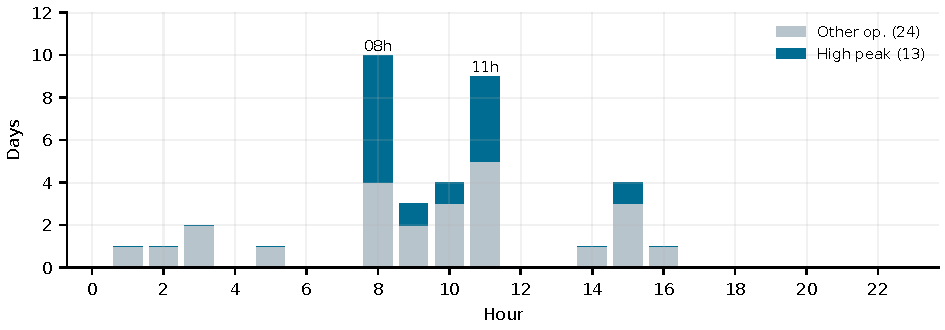
\includegraphics[width=\linewidth]{figs/peak_hours.pdf}
\caption{가동일의 첫 피크 시각 분포(개발 구간 37일). 짙은 색은 고피크일.}
\label{fig:ch3-peakhours}
\end{figure}

피크 시각은 08시와 11시에 몰린다(그림~\ref{fig:ch3-peakhours}). 가동일 37일 가운데 첫 최댓값이 08시인 날이 10일, 11시인 날이 9일이다. 고피크일 13일 중 10일(08시 6일, 11시 4일)이 이 두 시각에 피크를 기록했다. 피크가 생산이 있는 특정 시각에 생기므로, 생산계획을 입력으로 받아 시각별 부하를 예측하는 모델이 필요하다. 이 관계는 사후 연관이며 표본이 작다(고피크 13일).

\subsection{누수 진단과 검증 설계}

복사일이 섞인 자료에서 무작위 분할은 성능을 좋게 보이게 한다. 9월 이전 241일에 대해 날짜 단위 무작위 5-fold와 LOEO(leave-one-event-out)를 비교하였다. LOEO는 같은 복사 사건에 속한 날을 함께 빼며, 사건은 126개(복사군 45개, 단독일 81개)다. 비교 모델 M2(LightGBM 기본)의 MAE는 무작위 분할에서 14.91 kW, LOEO에서 16.64 kW였다(표~\ref{tab:ch3-leak}). 차이 $-1.73$ kW의 날짜 짝 부트스트랩 95\% 구간은 0을 포함하지 않는다. 기존 BAT는 두 분할에서 거의 같았다. 학습과 시험 사이의 중복 표본이 성능을 부풀리는 전형적인 누수다\citep{kapoor2023leakage}.

\begin{table}[h]
\centering
\caption{복사일 포함 자료에서의 누수 진단(MAE, kW, 241일).}
\label{tab:ch3-leak}
\begin{tabular}{lrrr}
\toprule
모델 & 무작위 5-fold & LOEO & 차이 [95\% 구간] \\
\midrule
M2(LightGBM 기본) & 14.91 & 16.64 & $-1.73$ [$-3.63$, $-0.04$] \\
기존 BAT & 16.37 & 16.32 & $+0.05$ [$-0.22$, $+0.42$] \\
\bottomrule
\end{tabular}
\end{table}

이 결과에 따라 모든 모델 비교는 복사일을 목표에서 뺀 시간순 분할로 한다. 시계열에서는 무작위 교차검증보다 시간 순서를 지키는 블록 분할이 적절하다\citep{roberts2017blockcv,bergmeir2018cv}. 검증 구간 f1--f4는 2021년 7월 7일부터 8월 31일까지 14일씩 네 구간이다. 각 구간의 모델은 그 이전 자료만으로 학습한다. 검증 첫날 전날은 간격일로 두어 목표에서 빼고 첫 검증일의 입력으로만 쓴다. 검증 구간과 같은 복사 사건에 속한 학습일은 제거(purge)하는 규칙을 두었으나, 실제로 해당하는 날은 없었다. 네 구간에서 유효하게 채점되는 표본은 53일, 5,016슬롯이고 일 피크 평가일은 51일이다. 확률 모형은 난수 시드 0, 1, 2로 반복 적합하고 시드별 점수를 평균한다. 시드 반복은 관측일 수를 늘리지 않는다.

9월 1--14일은 최종 평가 구간으로 봉인하였다. 기본 로더가 이 구간의 목표와 입력을 모두 가린다. 이 구간은 이전 개발 단계(v2)에서 열린 적이 있으므로 완전한 미사용 구간은 아니다. C-BAT는 개발 구간에서 확정·동결한 뒤 9월에 적용했으며 9월로 구조나 하이퍼파라미터를 선택하지 않았다. 이후 확장 실험도 f1--f4에서만 사전 등록 규칙으로 평가했다. 보고서의 주 성능은 개발 구간과 9월을 합친 67일·6,358슬롯, 피크 65일의 시간순 평가로 제시한다. 개발 구간은 모델 선택·절제·조건별 분석에, 9월 단독 결과는 기간별 차이 분석에 사용한다.
